%% Creator: Inkscape inkscape 0.48.0, www.inkscape.org
%% PDF/EPS/PS + LaTeX output extension by Johan Engelen, 2010
%% Accompanies image file 'FDL-setup.pdf' (pdf, eps, ps)
%%
%% To include the image in your LaTeX document, write
%%   \input{<filename>.pdf_tex}
%%  instead of
%%   \includegraphics{<filename>.pdf}
%% To scale the image, write
%%   \def\svgwidth{<desired width>}
%%   \input{<filename>.pdf_tex}
%%  instead of
%%   \includegraphics[width=<desired width>]{<filename>.pdf}
%%
%% Images with a different path to the parent latex file can
%% be accessed with the `import' package (which may need to be
%% installed) using
%%   \usepackage{import}
%% in the preamble, and then including the image with
%%   \import{<path to file>}{<filename>.pdf_tex}
%% Alternatively, one can specify
%%   \graphicspath{{<path to file>/}}
%% 
%% For more information, please see info/svg-inkscape on CTAN:
%%   http://tug.ctan.org/tex-archive/info/svg-inkscape

\begingroup
  \makeatletter
  \providecommand\color[2][]{%
    \errmessage{(Inkscape) Color is used for the text in Inkscape, but the package 'color.sty' is not loaded}
    \renewcommand\color[2][]{}%
  }
  \providecommand\transparent[1]{%
    \errmessage{(Inkscape) Transparency is used (non-zero) for the text in Inkscape, but the package 'transparent.sty' is not loaded}
    \renewcommand\transparent[1]{}%
  }
  \providecommand\rotatebox[2]{#2}
  \ifx\svgwidth\undefined
    \setlength{\unitlength}{226.77165527pt}
  \else
    \setlength{\unitlength}{\svgwidth}
  \fi
  \global\let\svgwidth\undefined
  \makeatother
  \begin{picture}(1,0.74999997)%
    \put(0,0){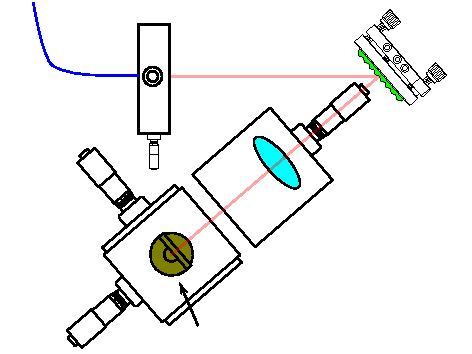
\includegraphics[width=\unitlength]{FDL-setup.pdf}}%
    \put(0.7880109,0.32385738){\color[rgb]{0,0,0}\makebox(0,0)[lb]{\smash{\fnurl{kinematic mount}{http://en.wikipedia.org/wiki/Mirror_mount}}}}%
    \put(0.60592285,0.21016686){\color[rgb]{0,0,0}\makebox(0,0)[lb]{\smash{$\begin{array}{c}
\text{XY linear}\\
\text{translator stage}
\end{array}$}}}%
    \put(1.05703259,0.22526822){\color[rgb]{0,0,0}\makebox(0,0)[lb]{\smash{$\begin{array}{c}
\text{1-Axis linear}\\
\text{translator stage}
\end{array}$}}}%
    \put(1.04513118,0.60704186){\color[rgb]{0,0,0}\makebox(0,0)[lb]{\smash{$\begin{array}{c}
\text{Diffraction}\\
\text{grating}
\end{array}$}}}%
    \put(0.46148539,0.50959389){\color[rgb]{0,0,0}\makebox(0,0)[lb]{\smash{Lens}}}%
  \end{picture}%
\endgroup
